% =====================================================================
%  TARIFF VERSUS GST — a standalone note for eventual inclusion in the
%  aluminium report. Not yet merged.
%  Every figure is produced by tariff_gst_arithmetic.py.
% =====================================================================
\documentclass[11pt, a4paper]{article}
\usepackage[a4paper, top=2.2cm, bottom=2.2cm, left=2.2cm, right=2.2cm]{geometry}
\usepackage{fontspec}
\IfFontExistsTF{DejaVu Sans}
  {\setmainfont{DejaVu Sans}}
  {\IfFontExistsTF{Verdana}{\setmainfont{Verdana}}{\setmainfont{Arial}}}
\usepackage{booktabs}
\usepackage{amsmath}
\usepackage{enumitem}
\usepackage{xcolor}
\usepackage{titlesec}
\usepackage{float}
\usepackage{tikz}
\usetikzlibrary{patterns, arrows.meta, calc}
\usepackage{tcolorbox}
\emergencystretch=2.5em
\hbadness=10000

\definecolor{g2}{gray}{0.88}
\definecolor{g4}{gray}{0.66}
\definecolor{shade}{gray}{0.945}
\newtcolorbox{keybox}{colback=shade, colframe=black!55, boxrule=0.5pt,
  arc=2pt, left=7pt, right=7pt, top=5pt, bottom=5pt}

\titleformat{\section}{\large\bfseries}{\thesection}{0.7em}{}
\titleformat{\subsection}{\normalsize\bfseries}{\thesubsection}{0.7em}{}
\setlength{\parskip}{0.35em}

\title{\textbf{Tariff or GST?}\\
\large The fiscal case for rationalising the duty on primary aluminium}
\author{}
\date{}

\begin{document}
\maketitle
\vspace{-1.0cm}

\begin{center}
\small\itshape A standalone note, for eventual inclusion in
\textit{Rationalizing Tariff Structures in the Indian Downstream Aluminium
Industry}. Every figure is reproduced by \texttt{tariff\_gst\_arithmetic.py},
which declares its baseline in one block and reports results across the
plausible range of each parameter.
\end{center}

\vspace{0.3cm}

\section{The argument, and what it rests on}

The objection that stops tariff rationalisation is fiscal: cutting the duty on
primary aluminium forgoes revenue. The answer has three parts, and they are of
descending robustness --- which is how they should be presented.

\textbf{First, and independent of any data: the two instruments are not
substitutes.} A customs duty on an intermediate input is a tax on production; GST is
a tax on consumption, creditable along the chain. Optimal-tax theory since Diamond
and Mirrlees holds that revenue should be raised on final uses and production left
undistorted. That is the distinction between these two instruments exactly.

\textbf{Second, and resting only on an identity: the duty is a very inefficient way
to raise the money.} Because domestic metal is priced at import parity, the duty
lifts the price of \emph{all} metal sold domestically while the exchequer collects
only on the imported fraction. The ratio of what is transferred to what is collected
is
\[
\frac{a}{c} \;=\; \frac{\phi\,(1-\mu)}{\mu\,(1-f)},
\]
where $\mu$ is import penetration, $\phi$ the pass-through of the duty into the
domestic price and $f$ the share of imports entering duty-free under trade
agreements. \textbf{No price, exchange rate or elasticity appears in it.} At the
baseline the ratio is \textbf{17.5 to 1}; across every corner of the parameter
ranges declared in §2 it runs from \textbf{5.5 to 39}. It is never near unity, and
that is the only thing the argument requires.

\textbf{Third, and resting on more assumptions: the sum at stake is trivial.} Net of
duty-free imports the duty raises about \textbf{INR 444 crore} --- 0.02 per cent of
FY26 gross GST collections, or under two hours of GST receipts. Replacing it exactly
would take \textbf{0.18 of a percentage point} on the GST rate applying to these
goods.

\begin{keybox}
\textbf{The mechanism.} The duty raises the marginal cost of every downstream
fabricator, because metal is bought at import-parity prices whether it is imported or
not. Removing it lowers that marginal cost. Since bought-in inputs are 83.1 per cent
of downstream output value, the relief is amplified roughly fivefold by the time it
reaches value added. That released margin is the space in which a marginally higher
consumption tax can be absorbed --- and the exchequer then taxes the larger base that
results.
\end{keybox}

\section{Baseline}

Every number in this note comes from the parameters below. Each is given with a
plausible range, and §6 reports how far the conclusions move across those ranges.

\begin{table}[H]
\centering
\footnotesize
\begin{tabular}{llllp{4.6cm}}
\toprule
& \textbf{Parameter} & \textbf{Baseline} & \textbf{Range} & \textbf{Source and remarks} \\
\midrule
B1 & Basic customs duty, HS 7601 & 7.5\% & --- & Tariff schedule \\
B2 & Social welfare surcharge & 10\% of BCD & --- & Levied on BCD; not creditable \\
& \textit{Effective pre-IGST duty} $t$ & \textit{8.25\%} & --- & Derived \\
B3 & GST / IGST on aluminium & 18\% & --- & Creditable; does not enter cost \\
\midrule
B4 & Domestic primary consumption $Q_C$ & 4.50 Mt & 3.5--5.0 & Industry data, CY2024 \\
B5 & Primary imports $Q_M$ (HS 7601) & 0.392 Mt & --- & Report §3.1, 2024 \\
& \textit{Import penetration} $\mu$ & \textit{8.7\%} & --- & Consistent with the reported ``under 10 per cent'' \\
B6 & Value of those imports & US\$1.03bn & --- & Report §3.1 \\
B7 & Exchange rate & INR 87/USD & 83--90 & Assumption \\
& \textit{Implied landed price} & \textit{INR 2.29 lakh/t} & --- & Derived from B5--B7 \\
\midrule
B8 & Duty pass-through $\phi$ & 1.00 & 0.70--1.00 & Import-parity pricing; $\phi=1$ is full parity \\
B9 & Duty-free share of imports $f$ & 40\% & 0--70\% & \textbf{The least certain parameter.} ASEAN, Japan and Korea rates are zero on most HS 7601 lines \\
\midrule
B10 & Supply elasticity $\varepsilon_s$ & 0.20 & 0.10--0.50 & Metals literature; primary supply is capital-constrained \\
B11 & Demand elasticity $|\varepsilon_d|$ & 0.50 & 0.20--0.80 & Metals literature \\
B12 & Metal share of downstream input bill $\theta$ & 60\% & 30--70\% & Not observable in the ASI \\
\midrule
& Amplification $m/(1-m)$ & 4.91 & --- & Report §4.7, $m = 0.8309$ \\
& Downstream output (ASI) & INR 2.46 lakh cr & --- & Three fabrication classes, 2022--23 \\
& Downstream GVA (ASI) & INR 41,653 cr & --- & 2022--23 \\
& FY26 gross GST collections & INR 22.27 lakh cr & --- & Official monthly releases \\
\bottomrule
\end{tabular}
\end{table}

\noindent Two of these deserve comment. \textbf{B9} is the weakest link: the exact
share of HS~7601 arriving duty-free is not published in the working data, and the
baseline of 40 per cent is an estimate. It is treated as a range throughout, and the
central result is reported at $f = 0$ as well. \textbf{B12} is not observable in the
ASI at all, which is why the induced-expansion calculation in §\ref{sec:offset} is
presented as a bound rather than an estimate.

\section{Why a duty and a consumption tax are not equivalent}

\subsection{Production efficiency: do not tax intermediate goods}

The governing result is the Diamond--Mirrlees production efficiency
theorem.\footnote{Diamond \& Mirrlees (1971), \textit{Optimal Taxation and Public
Production I: Production Efficiency} and \textit{II: Tax Rules}, American Economic
Review 61, 8--27 and 261--278.} Under standard conditions the optimal tax system
preserves productive efficiency: revenue should be raised on final uses, and
\emph{intermediate goods should not be taxed}. A tax on an intermediate input
distorts the technique of production as well as the level of consumption, so it does
two kinds of damage where a consumption tax does one.

A customs duty on HS~7601 is that instrument. Primary aluminium is not consumed; it
is an input to extrusion, rolling, casting and fabrication. Taxing it alters the
relative price of a produced input against labour, against capital, and against the
finished imported article, which is untaxed.

\subsection{Target the distortion at its source}

Bhagwati and Ramaswami established that where the objective concerns domestic
production, the first-best instrument acts directly on production; a trade instrument
is second-best, because it attains the production objective only by simultaneously
distorting consumption.\footnote{Bhagwati \& Ramaswami (1963), \textit{Domestic
Distortions, Tariffs, and the Theory of Optimum Subsidy}, Journal of Political
Economy 71(1), 44--50; see Panagariya (2006), The World Economy 29(10).} If the
objective is to sustain domestic smelting capacity, the theorem prescribes a
production subsidy, not an import duty.

\subsection{The decisive institutional difference: creditability}

One fact settles the comparison in practice. \textbf{IGST paid on imported metal is
creditable; basic customs duty is not.} A registered fabricator recovers the 18 per
cent IGST against output liability, so it never enters cost. The 8.25 per cent duty
is unrecoverable: it enters the cost base, is marked up at each subsequent stage, and
cascades. Two nominally similar levies therefore behave in opposite ways.

\section{Incidence: who gains and who pays}

\subsection{The diagram, with one adaptation}

Figure~\ref{fig:surplus} is the small-country tariff diagram applied to primary
aluminium. The adaptation that matters is on the demand side: the buyers of HS~7601
are not households but \emph{downstream producers}. What the textbook labels consumer
surplus is producer surplus in the fabrication sector --- the surplus whose employment
and wage consequences Section~4 of the report measures.

\begin{figure}[H]
\centering
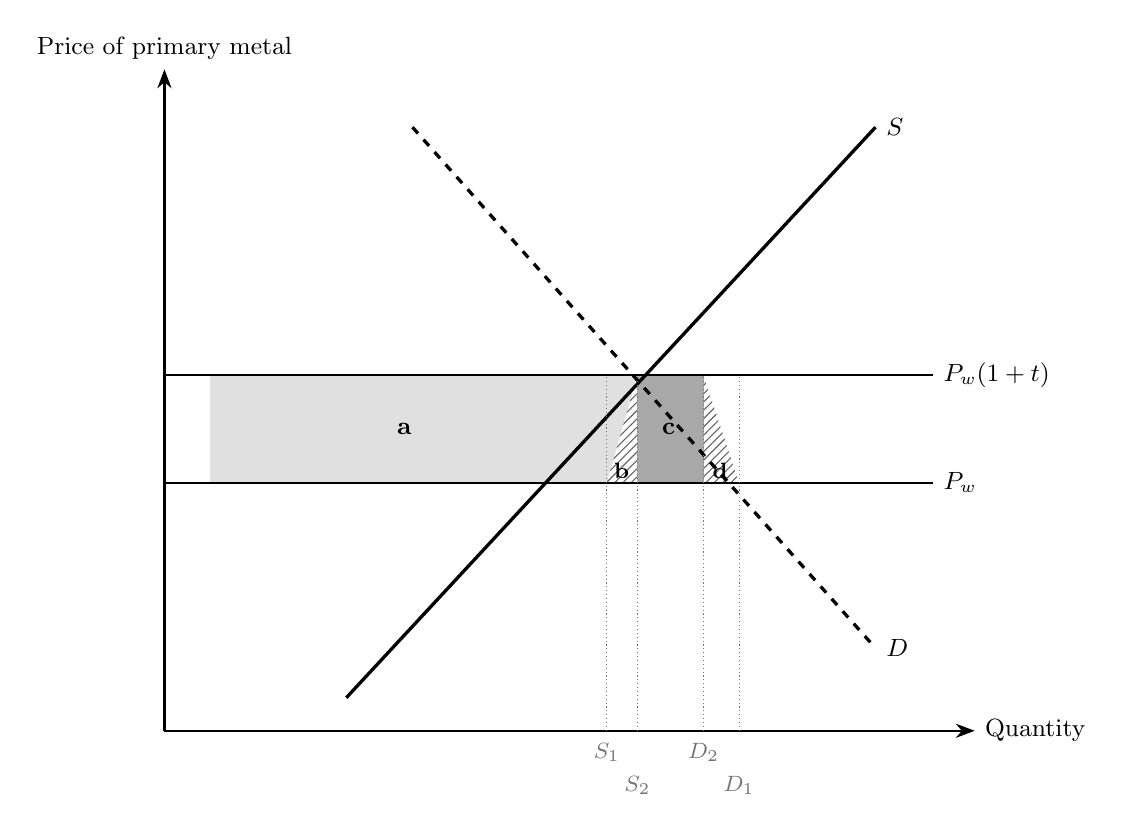
\begin{tikzpicture}[scale=1.05]
  \def\Pw{3.0}   \def\Pd{4.3}
  \def\Sa{5.35}  \def\Sb{5.72}
  \def\Db{6.52}  \def\Da{6.95}

  \fill[g2] (0.55,\Pw) -- (\Sa,\Pw) -- (\Sb,\Pd) -- (0.55,\Pd) -- cycle;
  \fill[pattern=north east lines, pattern color=black!60] (\Sa,\Pw) -- (\Sb,\Pd) -- (\Sb,\Pw) -- cycle;
  \fill[g4] (\Sb,\Pw) rectangle (\Db,\Pd);
  \fill[pattern=north east lines, pattern color=black!60] (\Db,\Pw) -- (\Da,\Pw) -- (\Db,\Pd) -- cycle;

  \draw[-{Stealth[length=2.4mm]}, thick] (0,0) -- (0,8) node[above, font=\small] {Price of primary metal};
  \draw[-{Stealth[length=2.4mm]}, thick] (0,0) -- (9.8,0) node[right, font=\small] {Quantity};

  \draw[very thick] (2.2,0.4) -- (8.6,7.3) node[right, font=\small\bfseries] {$S$};
  \draw[very thick, dashed] (3.0,7.3) -- (8.6,1.0) node[right, font=\small\bfseries] {$D$};

  \draw[thick] (0,\Pw) -- (9.3,\Pw) node[right, font=\small] {$P_w$};
  \draw[thick] (0,\Pd) -- (9.3,\Pd) node[right, font=\small] {$P_w(1+t)$};

  \node[font=\small\bfseries] at (2.9,3.65) {a};
  \node[font=\footnotesize\bfseries] at (5.53,3.15) {b};
  \node[font=\small\bfseries] at (6.1,3.65) {c};
  \node[font=\footnotesize\bfseries] at (6.72,3.15) {d};

  \draw[black!55, densely dotted] (\Sa,0) -- (\Sa,\Pd) node[below=1pt, font=\footnotesize] at (\Sa,0) {$S_1$};
  \draw[black!55, densely dotted] (\Sb,0) -- (\Sb,\Pd) node[below=13pt, font=\footnotesize] at (\Sb,0) {$S_2$};
  \draw[black!55, densely dotted] (\Db,0) -- (\Db,\Pd) node[below=1pt, font=\footnotesize] at (\Db,0) {$D_2$};
  \draw[black!55, densely dotted] (\Da,0) -- (\Da,\Pd) node[below=13pt, font=\footnotesize] at (\Da,0) {$D_1$};
\end{tikzpicture}

\vspace{0.2cm}
{\raggedright\small \textbf{a} --- surplus gained by upstream producers.
\textbf{c} --- duty collected. \textbf{b} and \textbf{d} --- deadweight loss.
Downstream producers lose \textbf{a $+$ b $+$ c $+$ d}; national welfare loses
\textbf{b $+$ d}. \textbf{The figure still flatters the duty}: it is drawn at an
import share of about 20 per cent for legibility, whereas the actual share is 8.7 per
cent, so area~c is in reality narrower still relative to area~a.\par}
\caption{The incidence of an input duty under import-parity pricing}
\label{fig:surplus}
\end{figure}

\subsection{The transfer-to-revenue ratio is an identity}

Areas $a$ and $c$ are each the price wedge multiplied by a quantity, so their ratio
depends only on quantities:
\[
a = \phi\, t\, P_w\,(Q_C - Q_M), \qquad
c = (1-f)\, t\, P_w\, Q_M
\qquad\Longrightarrow\qquad
\frac{a}{c} = \frac{\phi\,(1-\mu)}{\mu\,(1-f)} .
\]
Price, exchange rate and both elasticities cancel. What remains is import
penetration, pass-through and the duty-free share --- and only the last of these is
seriously uncertain.

\begin{table}[H]
\centering
\small
\begin{tabular}{lrrrr}
\toprule
\textbf{Import penetration $\mu$} & \textbf{$f=0\%$} & \textbf{$f=20\%$} & \textbf{$f=40\%$} & \textbf{$f=60\%$} \\
\midrule
5\% & 19.0 & 23.7 & 31.7 & 47.5 \\
\textbf{8.7\% (baseline)} & 10.5 & 13.1 & \textbf{17.5} & 26.2 \\
10\% & 9.0 & 11.2 & 15.0 & 22.5 \\
15\% & 5.7 & 7.1 & 9.4 & 14.2 \\
20\% & 4.0 & 5.0 & 6.7 & 10.0 \\
\bottomrule
\end{tabular}

\vspace{0.15cm}
{\raggedright\footnotesize Rupees transferred from downstream to upstream per rupee
collected, at $\phi = 1$. At $\phi = 0.7$ every cell falls by 30 per cent; the most
conservative cell in the table then becomes 2.8.\par}
\end{table}

\subsection{Levels, and the cost of raising a rupee this way}

\begin{table}[H]
\centering
\small
\begin{tabular}{llr}
\toprule
& & \textbf{INR crore} \\
\midrule
a & Upstream producer surplus gained & 7{,}747 \\
c & Duty collected, net of duty-free imports & 444 \\
& \quad at the statutory rate on every tonne & 739 \\
b & Production deadweight & 64 \\
d & Conversion forgone & 175 \\
\midrule
a$+$b$+$c$+$d & \textbf{Downstream surplus lost} & \textbf{8{,}430} \\
b$+$d & \textbf{National welfare lost} & \textbf{239} \\
\bottomrule
\end{tabular}
\end{table}

\noindent Two ratios follow, and they are the numbers worth quoting.

\begin{keybox}
For every rupee the exchequer collects through this duty:
\begin{itemize}[leftmargin=1.4em, itemsep=1pt, topsep=3pt]
\item \textbf{INR 17.5} is transferred from downstream margins to upstream margins; and
\item \textbf{INR 0.54} of value is destroyed outright, before counting the transfer.
\end{itemize}
A tax that destroys fifty-four paise of national income per rupee raised is an
expensive way to raise revenue on any view. The corresponding figure for a creditable
consumption tax on final goods is, by construction, far lower --- which is the
Diamond--Mirrlees point restated in rupees.
\end{keybox}

\section{Replacing the revenue}

\subsection{What has to be replaced}

\begin{table}[H]
\centering
\small
\begin{tabular}{lrr}
\toprule
& \textbf{Net of duty-free imports} & \textbf{At the statutory maximum} \\
\midrule
Revenue to replace & INR 444 crore & INR 739 crore \\
GST rate change on the downstream base & $+$0.18 pp & $+$0.30 pp \\
\quad i.e.\ from 18 per cent to & 18.18\% & 18.30\% \\
Share of FY26 gross GST collections & 0.020\% & 0.033\% \\
Days of GST collection & 0.07 & 0.12 \\
\bottomrule
\end{tabular}
\end{table}

\noindent The base used is the ASI output of the three fabrication classes,
INR 2.46 lakh crore. Applied to a wider aluminium-articles base the required change
would be smaller still.

\subsection{The induced-expansion offset}
\label{sec:offset}

Removing an 8.25 per cent duty on metal raises downstream value added by
$4.91 \times \theta \times t \times \phi$, where 4.91 is the amplification factor
established in the report:

\begin{table}[H]
\centering
\small
\begin{tabular}{lrrl}
\toprule
$\theta$ & \textbf{Value added released} & \textbf{GST at 18\% on it} & \textbf{vs INR 444 cr forgone} \\
\midrule
30\% & $+$12.2\% $=$ INR 5{,}062 cr & INR 911 cr & covers it twice over \\
45\% & $+$18.2\% $=$ INR 7{,}593 cr & INR 1{,}367 cr & covers it \\
60\% & $+$24.3\% $=$ INR 10{,}124 cr & INR 1{,}822 cr & covers it \\
70\% & $+$28.4\% $=$ INR 11{,}811 cr & INR 2{,}126 cr & covers it \\
\bottomrule
\end{tabular}
\end{table}

\begin{keybox}
\textbf{Quote this table carefully.} It is illustrative, not a forecast. It assumes
the relief is retained in the sector rather than competed away, that capacity exists
to convert it into output, and that no offsetting upstream contraction reduces the
GST base elsewhere. What it establishes is not that the swap certainly pays for
itself, but that plausible second-round effects are an order of magnitude larger than
the first-round loss. A fiscal objection to a measure of this size is not a serious
objection.
\end{keybox}

\section{Sensitivity}

The headline ratio was recomputed at every corner of the declared ranges for $Q_C$,
$\phi$, $f$ and the exchange rate: \textbf{$a/c$ runs from 5.5 to 39.2}, against a
baseline of 17.5. It does not approach unity anywhere in the parameter space, which
is the only property the argument depends on.

The absolute levels are less robust, as they should be. The transfer scales with
$\phi$ and with $Q_C$; the deadweight scales with the elasticities, which are drawn
from the international metals literature rather than estimated for India. The
deadweight figures should therefore be read as an order of magnitude --- but note that
they enter the argument only to make it \emph{stronger}, and omitting them entirely
still leaves the transfer-to-revenue ratio intact.

\section{Does the evidence support revenue recovery?}

Baunsgaard and Keen, on panel data for 117 countries over 32 years, find that
high-income countries recover fully from domestic taxes what they lose from trade
liberalisation; that middle-income countries show robust replacement, essentially
dollar-for-dollar in the long run; and that recovery is weakest among low-income
countries. They also find that the presence of a value-added tax has in itself made
it easier to cope with the revenue effects of
liberalisation.\footnote{Baunsgaard \& Keen (2010), \textit{Tax revenue and (or?)
trade liberalization}, Journal of Public Economics 94(9--10), 563--577.} India is a
middle-income economy with a mature, comprehensively administered VAT: it is squarely
in the category for which the evidence of full replacement is strongest.

\section{The counterarguments, and how far they go}

\subsection{Informality: the Emran--Stiglitz objection}

The most serious theoretical challenge to substituting VAT for trade taxes is Emran
and Stiglitz's.\footnote{Emran \& Stiglitz (2005), \textit{On selective indirect tax
reform in developing countries}, Journal of Public Economics 89(4), 599--623.} The
standard prescription is derived from models with no informal sector; once the VAT's
incomplete coverage is acknowledged, a revenue-neutral reduction in trade taxes
offset by higher VAT can reduce welfare, because the trade tax reaches activity the
VAT cannot.

The objection has force and should be stated rather than avoided. Two things limit
its application here. First, it concerns taxes on \emph{final consumption} where the
informal sector escapes the net; the instrument at issue is a tariff on an
\emph{intermediate input} bought overwhelmingly by registered factories and cleared
through customs. Diamond--Mirrlees applies to that case directly, and
Emran--Stiglitz does not displace it. Second, a border levy functions in part as a
withholding device on downstream informality --- Keen's argument --- but IGST at the
border already performs that function, and performs it without entering anybody's
cost base.\footnote{Keen (2008), \textit{VAT, tariffs, and withholding: Border taxes
and informality in developing countries}, Journal of Public Economics 92(10--11),
1892--1906.}

\subsection{The upstream adjustment}

Rationalisation is not costless upstream, and the note should not pretend otherwise.
Domestic realisations would fall towards import parity, and area~$a$ --- about
INR 7,750 crore on the baseline --- is the measure of what is lost. Two considerations
bound it: the segment is currently earning substantial operating surpluses and
expanding capacity, so the change compresses margin rather than threatening
viability; and a large share of Indian primary output is exported at world prices
already, and is unaffected.

\subsection{The trade-agreement constraint}

A reduction in the applied MFN rate extends to all partners, so the measure cannot be
targeted. That bears on \emph{how} to rationalise rather than whether: it points
towards a general reduction rather than a partner-specific one, and it is why the
report treats trade-remedy instruments as a separate question from the input duty.

\section{How to frame this in the report}

\begin{enumerate}[leftmargin=1.6em, itemsep=4pt]
\item \textbf{Lead with the identity, not the levels.} $a/c = \phi(1-\mu)/[\mu(1-f)]$
requires no price, no exchange rate and no elasticity. A reader can check it on the
back of an envelope, and there is nothing in it to dispute except import penetration,
which is published.

\item \textbf{Give the two per-rupee numbers together.} ``INR 17.5 transferred and
54 paise destroyed, per rupee collected'' is the sentence that carries the section.

\item \textbf{Put the instrument comparison before the arithmetic.} A reader who has
accepted that BCD sticks to cost while GST does not will accept what follows.

\item \textbf{Name the theorems.} Diamond--Mirrlees and Bhagwati--Ramaswami convert
what sounds like an industry request into the textbook treatment of an input tax.

\item \textbf{Concede the upstream loss and quantify it.} Area~$a$ is the concession.
Making it with a number attached is what distinguishes this from a lobbying document.

\item \textbf{State the Emran--Stiglitz objection first, then answer it.}

\item \textbf{Do not overclaim §5.2.} The defensible claim is that the sum at stake is
too small to be decisive --- not that reform is costless.
\end{enumerate}

\section{Suggested placement}

A new subsection in Section~5, immediately before the policy recommendations, running
to about a page and a half: the instrument comparison, the identity and its table,
the two per-rupee ratios, and the GST equivalence. The baseline table, the welfare
accounting, the sensitivity analysis and the counterargument discussion belong in an
appendix, consistent with the convention already adopted for the ASI material.

\section*{References}
\small
\begin{itemize}[leftmargin=1.2em, itemsep=2pt, label={}]
\item Baunsgaard, T. \& Keen, M. (2010). Tax revenue and (or?) trade liberalization.
\textit{Journal of Public Economics}, 94(9--10), 563--577.
\item Bhagwati, J. N. \& Ramaswami, V. K. (1963). Domestic distortions, tariffs, and
the theory of optimum subsidy. \textit{Journal of Political Economy}, 71(1), 44--50.
\item Diamond, P. A. \& Mirrlees, J. A. (1971). Optimal taxation and public
production I: production efficiency; II: tax rules. \textit{American Economic
Review}, 61, 8--27 and 261--278.
\item Emran, M. S. \& Stiglitz, J. E. (2005). On selective indirect tax reform in
developing countries. \textit{Journal of Public Economics}, 89(4), 599--623.
\item Keen, M. (2008). VAT, tariffs, and withholding: border taxes and informality in
developing countries. \textit{Journal of Public Economics}, 92(10--11), 1892--1906.
\item Panagariya, A. (2006). Bhagwati and Ramaswami: why it is a classic.
\textit{The World Economy}, 29(10).
\item Viner, J. (1950). \textit{The Customs Union Issue}. Carnegie Endowment for
International Peace, New York.
\end{itemize}

\end{document}
